\documentclass{article}%
\usepackage[T1]{fontenc}%
\usepackage[utf8]{inputenc}%
\usepackage{lmodern}%
\usepackage{textcomp}%
\usepackage{lastpage}%
\usepackage{geometry}%
\geometry{tmargin=1.5cm,lmargin=1.5cm,rmargin=1.5cm}%
\usepackage{amsmath}%
\usepackage{amsopn}%
\usepackage{breqn}%
\usepackage{mathtools}%
\usepackage{enumitem}%
\usepackage{xcolor}%
\usepackage{pgf}%
\usepackage{pgfplots}%
\usepackage{pdfpages}%
\usepackage{tabularx}%
\usepackage{float}%
\usepackage{tikz}%
\pgfplotsset{compat=newest}%
%
\title{LaTeXDocs CookBook}%
\author{Bence Balogh}%
\date{\today}%
\title{LaTeXDocs CookBook}%
\author{Bence Balogh}%
\date{\today}%
%
\begin{document}%
\normalsize%
\section{Charts}%
\label{sec:Charts}%

%
\subsection{TikZ}%
\label{subsec:TikZ}%
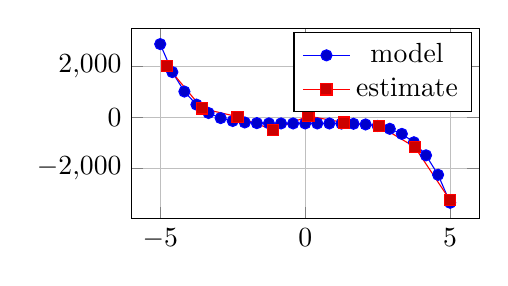
\begin{tikzpicture}%
\begin{axis}[height=4cm, width=6cm, grid=major]%
\addplot{-x^5 - 242};%
%
\addlegendentry{model}%
\addplot coordinates {%
(-4.77778,2027.60977)%
(-3.55556,347.84069)%
(-2.33333,22.58953)%
(-1.11111,-493.50066)%
(0.11111,46.66082)%
(1.33333,-205.56286)%
(2.55556,-341.40638)%
(3.77778,-1169.2478)%
(5.0,-3269.56775)%
};%
%
\addlegendentry{estimate}%
\end{axis}%
\end{tikzpicture}

%
\section{Matplotlib}%
\label{sec:Matplotlib}%

\begin{figure}[htp] \centering{
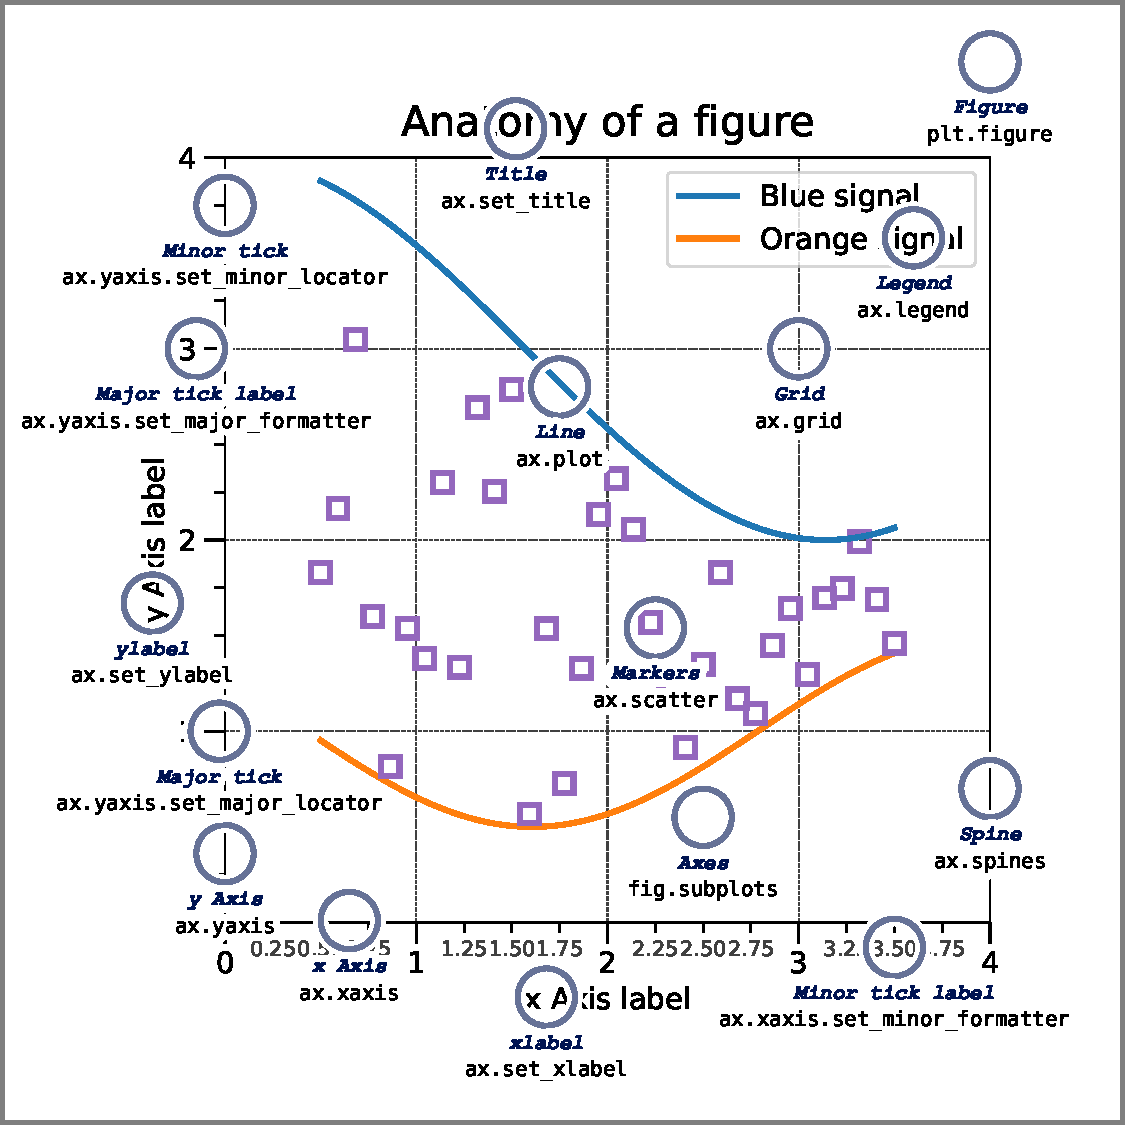
\includegraphics[scale=1.0]{mpl_anatomy.pdf}}
\caption{The anatomy of a matplotlib figure.}
\end{figure}  

%
\section{Tables}%
\label{sec:Tables}%
\begin{tabular}{|c|c|c|c|}%
\hline%
A&B&C&D\\%
\hline%
1&2&3&4\\%
5&6&7&8\\%
\hline%
\end{tabular}%
\newline%
\begin{tabularx}{\textwidth}{X|X|X|X}%
A&B&C&D \\ %
\hline%
1&2&3&4 \\ %
5&6&7&8 \\ %
\end{tabularx}

%
\end{document}